\subsection{Определяне на позиция в 3 измерения с помощта на трилатерация и приблизителни разстояния}

В източник \cite{murphy} е разработена система за следене на товарите в 3 измерения в мина чрез използване на трансмитери и получатели [фиг. \ref{fig:mine}]. Използвани са радио трансмитери. Разработен е специализиран лазер, който изчислява височината на товара, без който проблема за 3 измерения се е считал за нерешим. Проблем представляват разликите във височината и останалите измерения тъй като останалите измерения са в пъти по-големи в повечето случаи, както се вижда във фиг. \ref{fig:initPos}.

\begin{figure}
    \centering
    \centerline{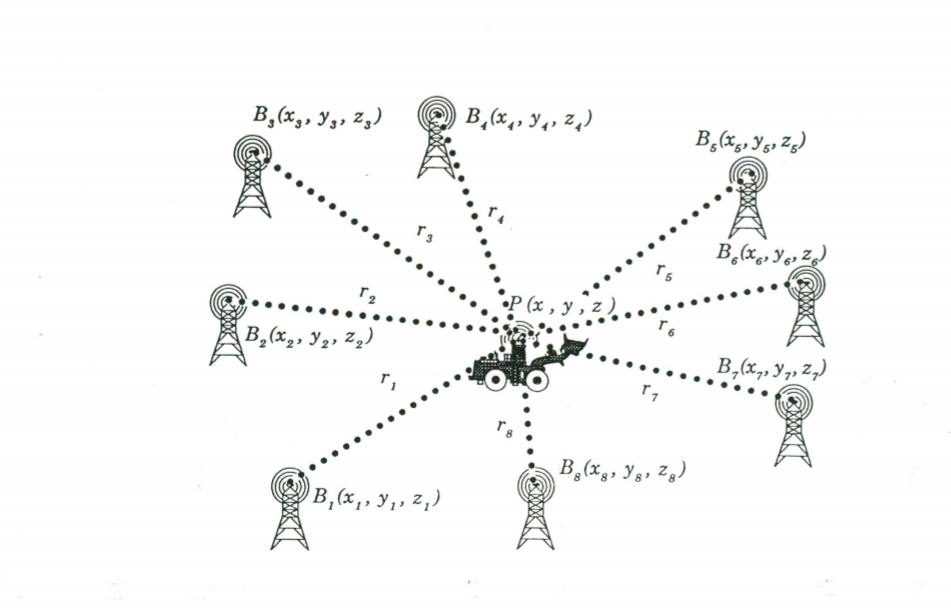
\includegraphics{dt1}}
    \caption{Разположение на получателите и предавателя в мина}
    \label{fig:mine}
\end{figure}

\begin{figure}
    \centering
    \centerline{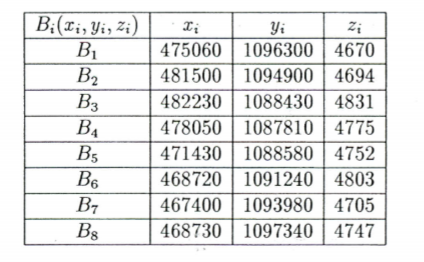
\includegraphics{MurphyInitialPositions}}
    \caption{Начално разположение на статичните получатели}
    \label{fig:initPos}
\end{figure}


\begin{equation}\label{circleEq}
    (x-x_i)^2 + (y-y_i)^2 +(z-z_i)^2=r_i^2
\end{equation}

Разглежда се възможността за съставяне система от \textit{N} на брой нелинейни уравнения използвайки формулата за сфера (израз \ref{circleEq}). Задачата се моделира като търсене на пресечни точки на N на брой сфери за всеки трансмитер.

Решението на гореспоменатата нелинейна система от израз \emph{се счита за не оптимално} тъй като полученото уравнение е нелинейно и е от висока степен. Когато разстоянията, които са измерени са точни, а не са приблизителни, линезирането на системата от уравнения е удачно. В този случай задачата се преобразува в търсенето на пресечната точка на няколко равнини.  \\

Разглежда се метод за линеризация на уравненията, за който всяка измерена дистанция между трансмитер и получател се използва уравнението за сфера ( кръг в 2D ) ( израз \ref{circleEq} ). Методът за линеризация съвпада с този използван в секция \ref{squares_algorithm}. Тъй като има (n-1) уравнения, за долна граница се считат 4 бр. приемника. Системи с по-малко от тази бройка приемници се считат за неизползваеми.
\\

Разглеждат се няколко метода за работа с приблизителни разстояния

\begin{itemize}
    \item \strong{Линейни най-малки квадрати} \\ Този метод предоставя по-задоволителни резултати в сравнение с решаване на проблема чрез решение на задачата с линеризиране на уравненията, но не дава оптимални резултати, защото резултатите определят координатите с  грешка повече от 5 фута ( работейки със измерените стойности в източник \cite{murphy}), което в ситуацията описана в източника, е недостатъчно като точност. Тъй като разстоянията са приблизителни се решава израз \ref{matrixeq}. Чрез минимизиране на сумата на квадратите на остатъците, израз \ref{nonNormalEq} води до израз \ref{normalEq}. \textit{[Noble and Daniel 1988]}
    
    \begin{equation} \label{matrixeq}
      A \vec{x} \approx \vec{b} 
    \end{equation}
    
    \begin{equation} \label{nonNormalEq}
        S = \vec{r}^T \vec{r} = (\vec{b} - A \vec{x})^T ( \vec{b} - A \vec{x})
    \end{equation}
    
    \begin{equation} \label{normalEq}
        A^T A \vec{x} = A^T \vec{b}
    \end{equation}
    
        
    Ако матрицата A в израз $A^T A$ на израз \ref{normalEq} e инвертируема се използва израз \ref{nonSing} , за да се намери решение на задачата.

    \begin{equation} \label{nonSing}
        \vec{x} = (A^T A)^{-1} A^T \vec{b}
    \end{equation}
	
	Ако матрицата не е инвертируема, се използва нормализирана QR-декомпозиция на \textit{A}. Задава се $A = QR$, където $Q$ е ортонормална матрица и $R$ е горно триангулярна матрица (всички стойности, които са над главния диагонал са 0). За намирането на търсения вектор $\vec{x} в нормализираната QR декомпозиция се използва израз \ref{QRDecEq}$.
    
	\begin{equation} \label{QRDecEq}
		R \vec{x} = Q^T \vec{b}
	\end{equation}
	
	Възможно е матрицата $A^T A$ да бъде близка до не инвертируема, въпреки че оригиналната матрица $A$ е инвертируема. За такива случай QR декомпозицията може да реши задачата. В случай, че решение не може да се намери с QR декомпозиция, singular value decomposition (SVD \cite{svd}) може да се използва, за да реши задачата.
	
    \item \strong{Нелинейни най-малки квадрати}\\
	Нелинейни най-малки квадрати дава най-добри резултати в сравнение с останалите изследвани методи. За минимизация на сумата на квадратите на грешките е известно, че трябва да се минимизира функцията в израз \ref{minimizeit}.
	
	\begin{equation} \label{minimizeit}
		F(x,y,z)=\sum_{i=1}^{n} (\hat{r_i} - r_i)^2=\sum_{i=1}^{n} f_i(x,y,z)^2
	\end{equation}\\
	
	където \\
	
	$f_i(x,y,z)=\hat{r_i}- r_i= \sqrt{(x-x_i)^2 = (y-y_i)^2 + (z-z_i)^2} - r_i$
	\\
	
	Проблемът за минимизация на сумата на квадратите на грешките е широко известен в сферата на приложната математика. В източник \cite{murphy} се използва метода на Нютон, ако се вземе предвид, че източника е от 1995, много от методите които се използват в днешно време не са описани.  Същата задача за минимизация се използва в линейната регресия, където той се решава чрез слизане по градиента (Gradient descent) \cite{lreg} с цел да се научи функция, която да предвижда стойности спрямо презадеден набор от данни в таблична форма.
    
\end{itemize}


\strong{Резултати}

\begin{figure}
    \centering
    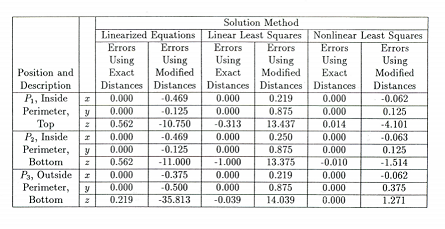
\includegraphics{murphyresults}
    \caption{Резултати при използване на различни методи за изчисление}
    \label{fig:murphyResults}
\end{figure}



Фиг. \ref{fig:murphyResults} демонстрира резултатите при определянето на координатите. Най-добри резултати се получават при използването на нелинейни най-малки квадрати, а най-лоши при използването на линеризирани уравнения. Линейните най-малки квадрати водят до най-добрите възможни за метода резултати, когато не съществува голяма разлика в стойностите на измеренията (x,y,z).